\documentclass[a4paper,12pt]{article}

%%%%%%%%%%%% PREÁMBULO %%%%%%%%%%%%%%%%%%%%%

% Paquetes

\usepackage{amsmath, amsthm, amssymb}
\usepackage[utf8]{inputenc}
\usepackage[spanish,es-tabla]{babel}
\usepackage[T1]{fontenc}
\usepackage{graphicx}
\usepackage{listings}
\usepackage{xcolor}
\usepackage{hieroglf}
\usepackage{bbding}
\usepackage{fancyhdr}

% Opciones
\chead{
\includegraphics[width=20cm]{fondo.jpg}}
\pagecolor{pink}
\begin{document}
\begin{titlepage}
\pagestyle{fancy}
	\centering

	{\scshape\LARGE Universidad la Salle \par}
	
\includegraphics[width=0.6\textwidth]{Estrella}\par

	\rule{80mm}{0.1mm}\\
	%\vspace{1.5cm}
	{\huge\bfseries HOMOMORFISMOS DE EVALUACIÓN\par}
	%\vspace{2cm}
	{\Large\itshape Autores:\par}
	{\Large\itshape Guillermo Aleman Zambrano\par}
	{\Large\itshape Daniela Vilchez Silva\par}
	\vfill
	\par
	%\vspace{0.5cm}
	{\Large\itshape Profesor:\par}
	{\Large\itshape Adeluz Apaza Valdivia \par}
	{\Large\itshape Algebra Abstracta\par}
	\vfill
	\vspace{2cm}
	{\Large\itshape 2019 - Arequipa Perú\par}

	\vfill

% Bottom of the page
%	{\large \today\par}
\end{titlepage}

%%%%%%%%%%%%%%%%%%%%%%%%%%%%%%%%%%%%%%%%%%%%%%

\textbf{¿Como se utiliza la maquinaria de homomorfismo y anillos factores para
resolver una ecuación polinomial?}

\tableofcontents

\section{Teorema de los homomorfismos de evaluación de la teoría de los campos.}


\begin{itemize}

    \item Definición:
     Sea F un subcampo de un campo E, sea $\alpha$ cualquier elemento de E y sea x una indeterminada. La transformación $\phi_\alpha:F[x]\longrightarrow E$ definida por \[ (a_0+a_1x+...+a_nx^n)\phi_\alpha =
     a_0+a_1\alpha+...+a_n\alpha^n     
\]
para $(a_0+a_1x+...+a_nx^n)$ $\epsilon$ $F[x]$ es un homomorfismo de $F[x]$ en E.
Además, $x\phi_\alpha = \alpha,$ y $\phi_\alpha$ transforma, de manera isomorfa, a F, mediante la 
transformación idéntica, esto es, $a\phi_\alpha = a $ para a $\epsilon$ F. El homomorfismo $\phi_\alpha$ es la \textbf{evaluación en }$\alpha.$
	\item Demostración:
	El diagrama reticular y de transformaciones, en la figura 30.1,
puede ayudar a visualizar esta situación. Las líneas punteadas indican un elemen­to del conjunto. En realidad, el teorema es una consecuencia inmediata de nuestras definiciones de suma y multiplicación en $F[x]$. Está claro que la trans­formación $\phi$ está bien definida, esto es, es independiente de nuestra representa­ción de $f(x)$ $\epsilon$ $F[x]$ como una suma finita.
\[ a_0+a_1x+...+a_nx^n\]
Dicha suma finita que representa a $f(x)$ puede modificarse sólo por la inserción y eliminación de términos $Ox^i$, lo cual, claramente, no afecta el valor de $(f(x))\phi_\alpha$.

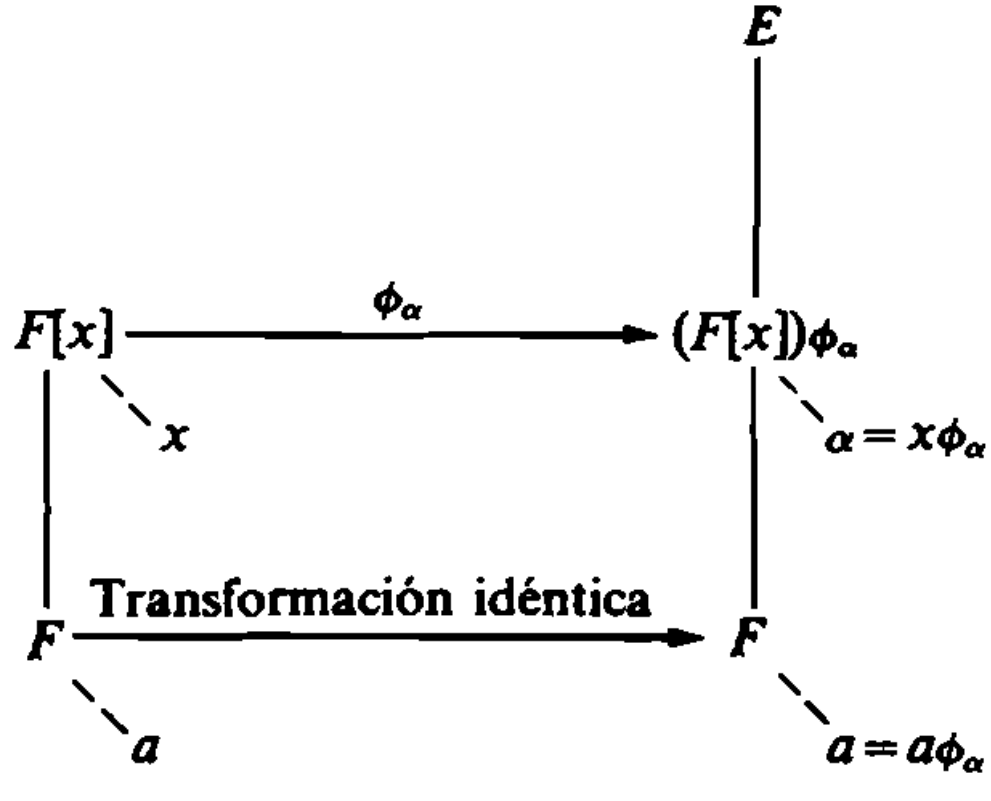
\includegraphics[width=0.7\textwidth]{imagen_latex.png}\centering

Si $f(x) = a_0+a_1x+...+a_nx^n$, 
$g(x) = b_0+b_1x+...+b_mx^m,$ y $h(x) = f(x)+g(x)=c_0+c_1x+...+c_rx^r$ entonces,
\[(f(x)+g(x))\phi_\alpha=(h(x))\phi_\alpha = c_0+c_1\alpha+...c_r\alpha^r,\]
mientras que

$(f(x))\phi_\alpha+(g(x))\phi_\alpha = (a_0+a_1\alpha+...+a_n\alpha^n)+(b_0+b_1\alpha+...+b_m\alpha^m)$
\end{itemize}

\end{document}